\documentclass[journal]{IEEEtran}
\usepackage[T1]{fontenc}
\usepackage{amsmath,amssymb,graphicx,booktabs,array,url}
\usepackage[hidelinks]{hyperref}
\graphicspath{{figures/}}
\begin{document}
\title{Feedback-Guided Classification Under Resource Constraints:\\A Reproducible General Algorithm SuperAgent}
\author{Group Authors and Affiliations to Be Completed%
\thanks{AIAA 3102 course project. Development draft, November 16, 2026. IEEE Transactions-style formatting does not imply journal submission or acceptance.}}
\markboth{AIAA 3102 COURSE PROJECT --- DEVELOPMENT DRAFT}{General Algorithm SuperAgent}
\maketitle
\begin{abstract}
We present a constrained classification SuperAgent combining LLM planning, train-only preprocessing, automatic validation selection, isolated fitting, and persistent usage accounting. The same frozen runtime and policy complete ten trials each on coupon-response prediction and ordered headline comparison. Final test accuracies are 79.0698\% and 66.8626\%. Each task makes nine DeepSeek-V4-Pro requests with returned usage; four plans are accepted and five truncated responses trigger deterministic fallback. Known current-run costs are CNY 0.2439945 and CNY 0.2704455 under the specified official off-peak rates. Historical Flash timeouts remain unreconciled, so the results are explicitly provisional development artifacts. Validation-prefix analysis shows an early coupon plateau and a small late headline gain, not guaranteed improvement from additional search. We document all candidate experiments, reproducibility evidence, submission coverage, and remaining limitations without inventing missing author or compliance information.
\end{abstract}
\begin{IEEEkeywords}Autonomous experimentation, classification, language models, reproducibility, resource accounting.\end{IEEEkeywords}
\section{Introduction}
\IEEEPARstart{A}{general} classification agent must inspect data, organize experiments, learn from feedback, select a solution, and produce a runnable model. With remote language models, reproducibility additionally requires verifiable identity and token accounting. A prediction file alone does not establish that these responsibilities have been met.

The AIAA 3102 assignment requires one SuperAgent across released and unseen tasks. Dataset names must not invoke manually prepared algorithms. Reported runs must be autonomous: students may develop the system beforehand but cannot edit code, decide subsequent experiments, or select a final model during execution~\cite{assignment}.

Our constrained agent combines an LLM planner with general executable menus, isolated fitting, automatic selection, refitting, and task-level usage records. It does not synthesize arbitrary executable code. This trades open-ended invention for traceability and bounded execution. The main contributions are shared modality-aware pipelines, structured feedback, strict final-only test access, and explicit separation of known usage from unresolved reservations.

This paper reports two complete ten-trial Pro development runs using the same frozen runtime and policy. Historical Flash requests still lack usage receipts. Thus, generated models are not accounting-complete formal submissions. Previous development also reused the designated test sets. Current run-level isolation does not restore project-wide independent evaluation.

\section{Requirements and Scope}
The assignment permits tabular, text, and image classification with task-specific formats, splits, and metrics. Eligible Qwen/DeepSeek models must have official releases on or before October 21, 2026, and official standard API pricing. Usage is capped at CNY 20 per reported task, including all agents; actual input/output tokens and costs must be recorded without cache discounts, promotions, or free-credit reductions. Local deployment does not remove accounting obligations~\cite{assignment}.

Grading covers released tasks (20\%), the unseen task (10\%), general design and autonomous development (30\%), execution/reproducibility/reporting (10\%), and presentation (30\%). This manuscript provides evidence for those categories without predicting grades. Image-related code and tests are not presented as a completed released image task.

The group must contain two to four students. Names, student identifiers, section, affiliations, and actual contributions remain to be supplied. No presentation or individual contribution is fabricated. The IEEE Transactions layout is a formatting choice, not a publication claim.

The assignment does not explicitly prescribe a single off-peak convention. We apply the requested off-peak accounting policy and disclose that instructor acceptance remains to be confirmed. Official model release dates also do not independently attest the exact school deployment revision.

\section{Architecture and Autonomous Workflow}
The unified entry point is \texttt{agent/main.py}, with train, predict, evaluate, freeze, and verify-freeze commands. Configuration validation checks feature roles, supported metrics and modalities, evaluation stages, and resource bounds. The data inspector excludes labels/IDs from inputs, validates partitions, and records hashes and split metadata.

Execution proceeds through configuration verification, environment capture, training/validation inspection, shared-ledger initialization, baseline fitting, iterative planning and validation, automatic selection, final refitting, and test prediction. Worker processes isolate fitting failures. The fitting cache excludes test data, and prediction has no feedback edge into search.

Data inspection, feature transformation, candidate construction, planning, fitting, orchestration, accounting, source freezing, and prediction are separate modules. Batch task names locate files and organize outputs; algorithm construction uses modality and generic statistics rather than dataset identity.

Fitted preprocessing and classification are serialized together with metadata. Pipeline and member cache dependencies are removed before saving. Inference therefore needs neither an original training cache nor an API key. Joblib artifacts should only be loaded from trusted sources.

\subsection{Selection and Refitting}
The first candidate establishes a class-prior baseline. Subsequent configurations come from a general planner and may be selected by an LLM using observed feedback. Successful candidates are ranked by metric utility:
\begin{equation}t^\star=\operatorname*{arg\,max}_{t\in\mathcal S}u(s_t),\end{equation}
where $s_t$ is validation performance and $\mathcal S$ contains successful trials. Accuracy is used for both tasks; it is not replaced by a more favorable metric.

After selection, the pipeline is refitted on training plus validation rows. If that fit fails, the next validation-ranked successful candidate may be attempted within the remaining deadline. Test scores never rank candidates. Final refitting uses 10,147 coupon rows and 9,241 headline rows.

A candidate cap operates alongside time/cost gates. Automatic devices allow CPU operation without CUDA. Recognizable out-of-memory failures can reduce batch size and then try CPU fitting; unrelated exceptions are not indiscriminately hidden. These are implemented recovery paths, not assertions that they all occurred here.

\section{Tasks and Evaluation Protocol}
Coupon acceptance is a binary task with 21 categorical inputs. Generic NumPy-to-CSV conversion creates $C_0$--$C_{20}$ and row IDs while preserving original partitions and row order. Numeric-looking categories remain categorical; no numeric columns are identified. Training labels contain 4,614 positives and 3,503 negatives. Missingness in $C_{11}$--$C_{15}$ is approximately 0.86\%--1.56\%, handled inside the fitted pipeline.

The headline task receives ordered \texttt{headline\_A} and \texttt{headline\_B}. Label one means A has higher CTR than B; zero denotes the reverse. Keeping A/B identity matters. Training labels contain 4,175 ones and 4,126 zeros; neither text column is missing.

\begin{table}[t]\centering\caption{Original supplied partitions.}\label{tab:data}
\begin{tabular}{lrrr}\toprule Task&Training&Validation&Test\\\midrule Coupon&8117&2030&2537\\ Headlines&8301&940&3232\\\bottomrule\end{tabular}\end{table}
Both tasks specify accuracy, $n^{-1}\sum_i\mathbf1[\hat y_i=y_i]$. Precision, recall and F1 are descriptive post-selection metrics. Test class statistics were read for reporting after execution, not passed to the planner. Every candidate uses the supplied validation partition.

The runs set \texttt{progressive\_output=false}: no intermediate test prediction is generated. The final model is selected and refitted before test conversion/inference/evaluation. Labels and test scores do not enter the menu or LLM context. This structural separation, timestamps, input hashes, and dedicated tests jointly support isolation; a boolean metadata flag alone is not proof. Earlier project-level test reuse remains a separate limitation.

\section{Features and Selected Models}
Tabular pipelines validate schemas, handle missingness, and accommodate unseen categories. CatBoost receives native categories; XGBoost uses train-fitted one-hot encoding. Other available families include linear models, forests, ExtraTrees, LightGBM, and neural networks when supported. Availability does not imply execution in every ten-trial run.

The selected coupon solution uses three CatBoost and three XGBoost members. CatBoost parameters are 1,200 iterations, depth eight, learning rate 0.05, and L2 leaf regularization five. XGBoost uses 1,600 iterations, depth six, learning rate 0.03, and regularization ten. Seeds start at 42 and differ by 101. Predictions combine groups as
\begin{equation}\hat p=\frac{0.75}{3}\sum_{j=1}^3p_j^{\mathrm{Cat}}+\frac{0.25}{3}\sum_{j=1}^3p_j^{\mathrm{XGB}}.\end{equation}
The selected leaf-model weight is zero. Identical members are cached across weight comparisons; later cache-hit timings are not intrinsic training complexity.

Text pipelines fit TF--IDF on allowed fitting data. Word features use one/two-grams, character features two- through five-grams. Combined features concatenate both. Separate-column representations preserve A/B identity; signed differences encode ordered contrasts. Length, punctuation, digits and uppercase counts are supplemental features.

Candidates include logistic regression, calibrated linear SVMs, neural models, and XGBoost after train-fitted 128-dimensional truncated SVD, bounded for small matrices. The selected headline solution is a three-fold calibrated linear SVM, $C=0.1$, combined word/character features, and separate-column representation. Calibration uses fitting data only. Calibration folds and ensemble members are not additional agent trials.
\section{LLM Planning and Reflection Evidence}
The school endpoint returns \texttt{DeepSeek-V4-Pro}. Request context includes modality, training-row/feature counts, class counts, missingness, available candidates, earlier scores, elapsed times and failure categories. Task names, dataset names, file paths and test information are excluded.

The response contract requires \texttt{choice}, \texttt{diagnosis}, \texttt{next\_action}, \texttt{abandoned\_strategy} and \texttt{reason}. Indices, repeated choices and required reflection fields are checked before execution. The model selects a reviewed action, not arbitrary generated code. Developer-designed menus and recovery policies remain substantive priors.

Each task issues nine Pro requests after its local baseline. All eighteen requests return actual usage without timeouts. Per task, four responses become accepted plans; five have \texttt{finish\_reason=length}, reach 2,048 completion tokens, lack valid complete JSON, and trigger deterministic fallback. HTTP-successful responses must not be counted as accepted decisions.

The auditable chain links raw requests/responses, accepted-plan or invalid-plan events, trial execution, measured feedback and final selection. Feedback records best utility before/after the candidate, with gain
\begin{equation}\Delta_t=\max_{k\leq t}u(s_k)-\max_{k<t}u(s_k).\end{equation}
A family with repeated failures may leave the menu, but all twenty current candidates succeed. An observed failure-driven abandonment episode is therefore not invented.

Richer logs expose what happened instead of manufacturing missing reasoning. Increasing output allowance or reducing context redundancy may improve valid-plan yield, but a new complete experiment has not established that benefit. The system's constrained autonomy is more limited than unrestricted self-programming.

\section{Experimental Setup and Histories}
Both runs share one frozen runtime and policy: ten candidates, seed 42, four threads, automatic device selection, a 7,200-second task budget, a 600-second trial allocation and final-fit reserve fraction 0.3. API timeout is 180 seconds and output allowance 2,048 tokens. CUDA is available, without requiring a specific personal device model.

Recorded software includes Python 3.11.15, NumPy 2.4.6, pandas 3.0.3, scikit-learn 1.9.0, SciPy 1.17.1, joblib 1.5.3, CatBoost 1.2.10, LightGBM 4.7.0 and XGBoost 3.2.0. These versions are audit facts, not universal requirements.

The appendix lists all twenty candidates and parameters. All succeed. Worker seconds include fitting/validation but exclude some API waiting, startup and orchestration. End-to-end training workflows record 1,183.375 seconds for coupons and 887.906 seconds for headlines, approximately 19.72 and 14.80 minutes; these are not pure GPU times.

The coupon model is selected at trial three and the headline model at trial nine. No human chooses the next candidate or final model inside these completed runs. Development edits before freezing and document preparation afterward are distinct activities. Fixed seeds improve reproducibility but do not guarantee identical remote-model responses.

\section{Results and Search-Budget Returns}
\begin{table}[t]\centering\caption{Final test results from one shared development runtime.}\label{tab:results}
\begin{tabular}{lrrr}\toprule Task&Correct/total&Accuracy (\%)&Macro-F1\\\midrule Coupon&2006/2537&79.0698&0.7841\\ Headlines&2161/3232&66.8626&0.6686\\\bottomrule\end{tabular}\end{table}
The coupon model predicts 2,006 of 2,537 examples correctly; the headline model predicts 2,161 of 3,232. Coupon class-zero/one recalls are 0.7142/0.8488; headline recalls are 0.6446/0.6935. These descriptive values suggest error-analysis directions but do not establish a semantic explanation for individual failures. A systematic error taxonomy has not been completed.

We compare prefixes of the same ten-trial path instead of re-evaluating the test set for each budget. Coupon best validation accuracy is 75.8128\% after two trials and 75.9606\% after five, eight and ten. The true best occurs at trial three; seven later candidates do not improve it. The gain over the two-trial prefix equals three validation examples.

Headlines remain at 69.0426\% through prefixes two, five and eight, then reach 69.1489\% by ten because of trial nine. This equals one extra correct validation example. Figure~\ref{fig:curve} distinguishes candidate scores from retained maxima. No repeated-seed or statistical-significance study supports stronger claims.

\begin{figure*}[t]\centering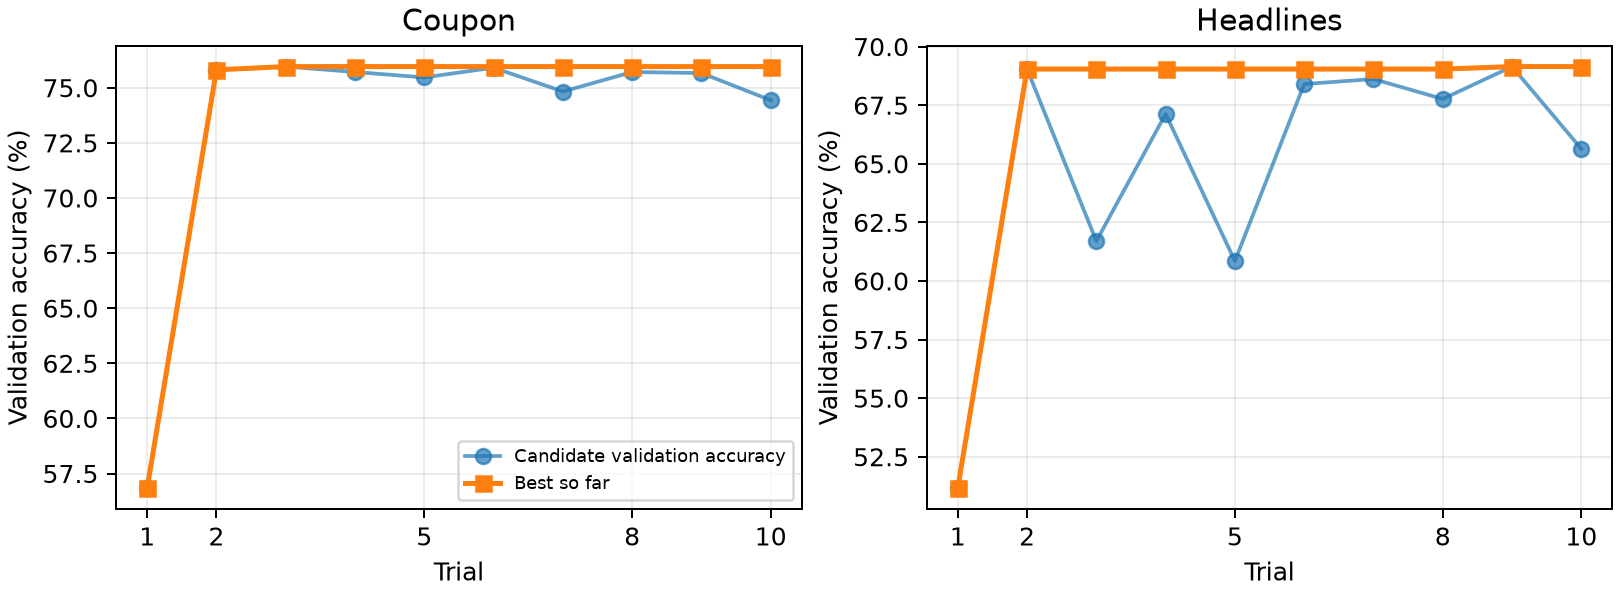
\includegraphics[width=.94\textwidth]{validation_curves.png}\caption{Candidate validation scores and retained maxima. This is one trajectory per task, not independent experiments for each prefix. The retained maximum cannot decrease by construction; generalization need not improve.}\label{fig:curve}\end{figure*}
The earlier two-trial API workflow produced coupon/headline test accuracies of 79.2274\%/66.0582\%. The present headline score rises while coupon falls. This is not a controlled Flash-versus-Pro comparison: trajectories and conditions differ, and test data were reused. Historical best artifacts remain separate, not substituted into this paper's unified pair.

No fifteen-trial comparison is complete under this policy. The evidence does not establish that fifteen trials beat ten, that more trials always improve test performance, or that Pro is intrinsically a better planner. Additional candidates can consume resources and overfit validation data without improving generalization.

\section{Token Usage and Budget Accounting}
The official historical image states Pro off-peak rates of CNY 4.5 per million input tokens (cache miss) and CNY 13.5 per million output tokens, effective August 17, 2026~\cite{prorelease,priceimage}. All input is priced at the cache-miss rate without platform discounts. Observed cost is
\begin{equation}C=\frac{4.5n_{\mathrm{in}}+13.5n_{\mathrm{out}}}{10^6}.\end{equation}
Output totals include reasoning when included in returned completion usage. Counts are not inferred from response-text length. Calculated values are accounting figures, not verified school invoices.

\begin{table}[t]\centering\caption{Known costs and unresolved holds (CNY).}\label{tab:cost}
\begin{tabular}{lrr}\toprule Quantity&Coupon&Headlines\\\midrule Current Pro run&0.2439945&0.2704455\\ Known task-wide total&0.3014195&0.2839105\\ Historical unknown hold&5.2428800&5.2428800\\ Actual complete total&Unknown&Unknown\\\bottomrule\end{tabular}\end{table}
Earlier Flash read timeouts retain unknown usage. A later successful connection does not establish that those requests were unprocessed. Each task holds CNY 5.24288; actual cumulative totals remain null. Records are not deleted, converted to zero or moved into a newly named task to restore budget.

An earlier DNS failure was separately reconciled using its original local getaddrinfo evidence of pre-connection failure. That reasoning does not apply to read timeouts. Provider usage receipts, or explicit confirmation that requests were not processed, are still needed.

The development-only mode includes known observed costs, existing unknown holds and the next worst-case hold in the CNY 20 check. Pro bounds are conservatively 1,048,576 input and 393,216 output tokens, using the reviewed official output limit~\cite{pricing}. Thus, the next-request hold is
\begin{equation}R=\frac{4.5(1048576)+13.5(393216)}{10^6}=10.027008.\end{equation}
This is not average or actual usage. Ambiguous requests are not retried and their holds remain; local planning may continue. Formal released/unseen execution rejects provisional accounting and requires reconciled actual usage.

Known costs plus historical holds are approximately CNY 5.5443/5.5268, below the bound but not actual complete totals. The summary therefore retains \texttt{accounting\_provisional=true} and \texttt{eligible\_for\_formal\_submission=false}. Generating predictions does not waive these formal prerequisites.

\section{Reliability, Isolation and Reproducibility}
Worker processes enforce native thread settings and candidate deadlines. Recognizable allocation errors can reduce batch size and then attempt CPU fitting, but unrelated failures are preserved. No actual OOM episode is claimed in these runs. Cached ensemble members explain some large trial-time differences.

Forty-two implementation checks pass. A dedicated strict-default check verifies that first prediction-time test access follows final selection and that no partial-test event occurs. This complements source structure, hashes and logs; none alone proves project-wide evaluation independence.

Copied models reproduce saved predictions row by row; probabilities also match. Training-cache paths are disconnected before serialization. Package hashes support copy-integrity checking. Report edits do not alter the immutable source snapshot, rerun models or rewrite original history.

Both models share this runtime SHA-256, shown as contiguous halves:
\begin{quote}\footnotesize\ttfamily d129aaae4c89df8f925759e30fd48a291\\60bfb774b592aadee6ae4d335d4d13e\end{quote}
Dependencies, hardware numerics, remote service behavior and aliases can change. Seeds do not guarantee bitwise equivalence or identical future LLM text. A generic school Pro response name does not attest its exact revision. Official release evidence and deployment identity are distinct.
\section{Installation and Fixed-Model Replay}
Install root \texttt{requirements.txt} in an appropriate Python environment. GPU training dependencies are described separately. Existing models support CPU inference without API keys. Only trusted joblib artifacts should be deserialized.

Verify the immutable snapshot with:
\begin{quote}\small\ttfamily python agent/main.py verify-freeze\\--manifest agent/frozen\_manifest.json\end{quote}
Coupon inference is:
\begin{quote}\small\ttfamily python agent/main.py predict\\--model tasks/coupon/model.joblib\\--input data/coupon/test.csv\\--output coupon\_predictions\_new.csv\end{quote}
For headlines, replace both task directories with \texttt{headlines} and choose a new output filename. Targets must not exist. Final evaluation uses the separate \texttt{evaluate} command on a fixed model and labeled input; the result must not become subsequent search feedback.

Fresh training requires correct local inputs, the intended algorithm policy, evaluation stage, local credentials and a ledger shared by all agents for that task. Historical paths in original records are audit evidence, not commands to rewrite into a fictitious new execution. The provisional option must not silently replace formal execution.

Fixed-model replay is available immediately. Formal retraining still requires historical receipts, deployment confirmation and an accepted price interpretation. Changing a configuration label does not convert development artifacts into compliant formal results.

\section{Unseen-Task Plan}
The course releases the unseen task after both sections finish presentations. The submitted SuperAgent must operate within 24 hours of release using its final frozen version, without human intervention. Predictions and execution logs are required, but no additional report~\cite{assignment}. No unseen score, duration or completion claim is currently available.

The intended process validates official formats, labels, metrics and release time, then applies the same frozen analysis, planning, validation, selection, refitting and prediction pipeline. Input configuration must not act as dataset-specific algorithm dispatch. Formal execution retains strict test isolation, verified eligibility and reconciled accounting.

Closing intermediate test access creates a real trade-off: a premature search termination may leave no test prediction. Partial work must be described honestly rather than filled with invented results. Support in source/tests does not establish empirical success on arbitrary large image datasets, multiclass problems or all malformed inputs. Those studies remain future work.

\section{Limitations and Future Work}
The system is constrained AutoML--agent integration, not unrestricted self-programming. Menus, priorities and recovery rules encode human choices. Eight of eighteen responses become accepted plans. Attributing all gains to LLM reasoning would overstate autonomy.

The principal observed planning defect is truncation at 2,048 tokens. Larger output allowance, shorter context or supported reasoning controls should be assessed by valid-JSON yield, cost and validation benefit. More elaborate logs alone do not improve decisions. These suggestions are not completed experiments.

Validation gains are small: three coupon examples and one headline example beyond the two-trial prefix. Repeated seeds, controlled planner ablations, confidence intervals and systematic error analysis are absent. Search may overfit fixed validation data, and prior test reuse adds selection bias.

The accounting and deployment gaps are substantive. The group must recover receipts for old timeouts, verify Pro's deployed revision and confirm acceptance of off-peak pricing. Low known costs do not replace complete actual accounting. Formal compliance is not claimed before those issues are resolved.

Further experiments should address those prerequisites and output failures before claiming broader generality or increasing search indefinitely. The observed plateau does not justify a universal recommendation for higher trial caps.

\section{Contributions and AI-Tool Disclosure}
\textit{To be completed by the group: member names, student IDs, section, affiliations, actual contributions and individual review statements.} Possible responsibility categories are data processing, orchestration, modeling, accounting/reproduction and reporting/presentation. They are suggestions, not invented claims about identified members.

OpenAI Codex assisted requirement interpretation, coding, review, debugging, testing and document preparation. Runtime school-model calls are recorded separately. The project ledger cannot establish developer-tool usage. Members should disclose additional tools and their own verification scope. This draft is not a signed statement on behalf of unidentified authors.

All members remain responsible for explaining the implementation, costs, results and limitations. Development assistance is distinct from autonomous execution. No final presentation or personal contribution is fabricated.

\section{Submission Coverage and Outstanding Actions}
The package contains runtime source and unified entry, dependencies/README, per-task models and results, experimental/resource logs, this report and editable LaTeX source, and an AI-tool statement. The appendix maps requirements to files.

Before final submission, complete authorship details, recover receipts, confirm deployment eligibility and pricing, and determine whether reconciled formal reruns are necessary. Report results must agree with the submitted code, models and logs. Completing report prose does not resolve experimental defects.

The deadline is 23:59 on the evening before the first class of the relevant section's final week; the section-specific date still requires confirmation. The submitted version is frozen for unseen evaluation. This manuscript covers the required topics without pretending unresolved facts are complete.

\section{Conclusion}
The shared agent completes ten trials and final inference for both released tasks using Pro-assisted decisions and auditable fallback. Copied artifacts reproduce stored predictions. Validation-prefix analysis shows an early coupon plateau and a small late headline gain, not guaranteed test improvement from additional trials.

Its strongest evidence is traceability across candidates, accepted plans, fallback, observed usage and unknown reservations. Restricted autonomy, output truncation, small unreplicated gains, reused tests and unresolved accounting/deployment evidence limit the conclusions. These are development results until the outstanding formal prerequisites are met.

\appendices
\section{Complete Candidate Histories}
The following tables retain every executed candidate, including those that do not improve validation. All twenty trials succeed. Times are worker fitting/validation measurements, not full workflow costs. Selected models remain the automatically chosen trial-three coupon blend and trial-nine headline SVM.
\begin{table*}[t]\centering\scriptsize
\caption{Complete coupon history. All candidates succeeded.}\label{tab:coupon}
\begin{tabular}{rp{0.66\textwidth}rr}\toprule Trial&Candidate and parameters&Validation (\%)&Seconds\\\midrule
1&family=dummy&56.8473&2.62\\
2&family=cross\_boost\_blend&75.8128&359.75\\
3&family=cross\_boost\_blend, gpu\_seeds=3, gpu\_weight=0.25, leaf\_weight=0.0&75.9606&15.47\\
4&family=cross\_boost\_blend, gpu\_seeds=3, gpu\_weight=0.5, leaf\_weight=0.0&75.7143&4.62\\
5&family=cross\_boost\_blend, gpu\_seeds=3, gpu\_weight=0.25, leaf\_weight=0.15&75.4680&5.53\\
6&family=cross\_boost\_blend, gpu\_weight=0.1&75.9113&3.67\\
7&family=catboost, iterations=600, depth=6, learning\_rate=0.05, l2\_leaf\_reg=3&74.8276&27.20\\
8&family=cross\_boost\_blend, gpu\_weight=0.5&75.7143&4.09\\
9&family=cross\_boost\_blend, gpu\_weight=0.75&75.6650&4.36\\
10&family=xgboost, iterations=2000, depth=4, learning\_rate=0.03, reg\_lambda=10&74.4335&6.58\\
\bottomrule\end{tabular}
\end{table*}
\begin{table*}[t]\centering\scriptsize
\caption{Complete headlines history. All candidates succeeded.}\label{tab:headlines}
\begin{tabular}{rp{0.66\textwidth}rr}\toprule Trial&Candidate and parameters&Validation (\%)&Seconds\\\midrule
1&family=dummy&51.1702&2.03\\
2&family=logistic, C=1.0, analyzer=char, representation=separate, class\_weight=balanced&69.0426&14.14\\
3&family=xgboost, iterations=1000, depth=3, learning\_rate=0.03, reg\_lambda=10, analyzer=combined, representation=separate, svd\_components=128&61.7021&15.05\\
4&family=linear\_svm, C=1.0, analyzer=char, representation=difference&67.1277&42.24\\
5&family=xgboost, iterations=1000, depth=6, learning\_rate=0.03, reg\_lambda=10, analyzer=combined, representation=separate, svd\_components=128&60.8511&7.36\\
6&family=linear\_svm, C=0.1, analyzer=char, representation=difference&68.4043&10.05\\
7&family=linear\_svm, C=0.1, analyzer=char, representation=separate&68.6170&34.22\\
8&family=linear\_svm, C=1.0, analyzer=char, representation=separate&67.7660&96.58\\
9&family=linear\_svm, C=0.1, analyzer=combined, representation=separate&69.1489&40.62\\
10&family=linear\_svm, C=10.0, analyzer=char, representation=difference&65.6383&57.22\\
\bottomrule\end{tabular}
\end{table*}\section{Artifact and Audit Index}
\begin{table*}[t]\centering\small\caption{Submission requirement coverage. File presence does not resolve compliance gaps.}\label{tab:files}
\begin{tabular}{p{.24\textwidth}p{.68\textwidth}}\toprule Requirement&Evidence\\\midrule
Complete code / entry&\texttt{agent/main.py}, \texttt{agent/superagent/}, immutable frozen manifest.\\
Dependencies / setup&Root \texttt{requirements.txt}, \texttt{requirements-gpu.txt}, \texttt{README.md}.\\
Runnable task solutions&Per-task \texttt{model.joblib}, \texttt{predictions.csv}, \texttt{test\_evaluation.json}.\\
Decisions and experiments&\texttt{trials.jsonl}, \texttt{events.jsonl}, original \texttt{model\_calls/}.\\
Resources and model evidence&\texttt{usage.jsonl}, \texttt{model\_usage.json}, \texttt{task\_model\_calls.json}, \texttt{environment.json}, official evidence snapshots.\\
Report and disclosure&\texttt{report.pdf}, \texttt{latex\_source/report.tex}, \texttt{AI\_USAGE.md}, \texttt{TODO\_BEFORE\_SUBMIT.md}.\\
Replay integrity&Root \texttt{verification.json}, \texttt{PACKAGE\_HASHES.json}, fixed \texttt{data/} partitions.\\\bottomrule\end{tabular}\end{table*}
Usage snapshots include previous attempts. Identify current-run calls by the summary's run ID. Unknown usage is not a zero-cost success; a hold is not a charge; validation is not test performance; an HTTP success is not necessarily an accepted plan. These distinctions are necessary to reproduce totals and avoid overstating autonomy.

\begin{thebibliography}{9}
\bibitem{assignment} AIAA 3102, ``Final Project: General Algorithm SuperAgent---Full Assignment Requirements,'' course-provided specification, included in the submission.
\bibitem{prorelease} DeepSeek, ``DeepSeek-V4-Pro official release,'' Aug. 13, 2026. [Online]. Available: \url{https://api-docs.deepseek.com/zh-cn/news/news260813/}
\bibitem{priceimage} DeepSeek, ``DeepSeek-V4 API pricing,'' historical official image, effective Aug. 17, 2026. [Online]. Available: \url{https://api-docs.deepseek.com/zh-cn/img/v4_260813_price_cn.png}. A hash-checked copy is included.
\bibitem{pricing} DeepSeek, ``Models and pricing,'' official documentation, snapshot retrieved Nov. 16, 2026. [Online]. Available: \url{https://api-docs.deepseek.com/zh-cn/quick_start/pricing/}. This does not attest the school deployment revision.
\end{thebibliography}
\end{document}
